\documentclass[12pt,a4paper,]{report}

\usepackage[T1,T8K,T8M]{fontenc}
\usepackage[utf8]{inputenc}
\usepackage[english,georgian]{babel}

\usepackage{graphicx}
\usepackage{hyperref}
\usepackage{mathtools}
\usepackage{gensymb}

\usepackage{subfig}

%\renewcommand{\rmdefault}{cmtt}

\hypersetup{
	pdftitle={dummy},
	pdfauthor={Levan Kankadze},
	bookmarksnumbered=true,     
	bookmarksopen=true,         
	bookmarksopenlevel=1,       
	colorlinks=true,
	linkcolor=blue,            
	pdfstartview=Fit,           
	pdfpagemode=UseOutlines,    
	%pdfpagelayout=TwoPageRight
}

\textwidth=16.5cm
\textheight=25cm
\voffset=-2.5cm
\hoffset=-2cm

 %ტექსტის გვერდების გასწორება
\tolerance=10000
\hyphenpenalty=100

\begin{document}

\begin{titlepage}
   \begin{center}
       \vspace*{1cm}

       \textbf{რადიაციული თერაპია}

       \vspace{0.5cm}
        Thesis Subtitle
            
       \vspace{1.5cm}

       \textbf{}

       \vfill
            
%       A thesis presented for the degree of\\
%       Doctor of Philosophy
            
       \vspace{0.8cm}
     
       
\includegraphics[width=0.4\textwidth]{images/kiu_logo}
            
       ქუთაისის საერთაშორისო უნივერსიტეტი\\
       საქართველო\\
       2021
            
   \end{center}
\end{titlepage}


\chapter{შესავალი}
მცირე შესავცალი რადიაციულ თერაპიაში.

\pagebreak

\chapter{რა არის რადაციული თერაპია?}
რადიაციული თერაპია არის სიმსივნის მკურნალობის მეთოდი, თუმცა დღესდღეობით რადიაციული თერაპიით შესაძლებელია სხვა დაავადებების განკურნებაც (გული, ...). რადიაციული თერაპია იყენებს ინტენსიური ნაკადების (დამუხტული ნაწილაკების ანდა ელექტრომაგნიტური გამოსხივების) ენერგიას სიმსივნის უჯრედების გასანადგურებლად. ხშირად რადიაციული თერაპია იყენებს რენტგენის სხივებს, თუმცა პროტონების ან სხვა დამუხტული ნაწილაკების გამოყენებაც შეიძლება.

ტერმინი \textbf{რადიაციული თერაპიას} ხშირად ეძახიან  გარე ნაკადებით დასხივებას. ამ ტიპის დასხივებისას, მაღალი ენერგიის ნაკადები გამომსხივებელი მოწყობილობიდან ეცემა სხეულის რომელიმე წინასწარ ზუსტად განსაზღვრულ წერტილს. არსებობს სხვა ტიპის რადიაციული თერაპიას, მაგალითად \textbf{ბრაქითერაპია}\cite{brachytherapy} ამ დროს გამომსხივებელი არის მოთავსებული სხეულის შიგნით. 

რადიაციული თერაპია აზიანებს უჯრედების გენეტიკურ მასალას, რაც პასუხისმგებელია უჯრედის ზრდასა და გაყოფაზე. ცხადია რადიაციულ თერაპია აზიანებს ორივე ჯანმრთელსა და სიმსივნურ უჯრედებს. რადიაციული თერაპიის მიზანია რაც შეიძლება მცირე რაოდენობის ჯანმრთელი უჯრედი დაზიანდეს დასხივებისას. ჯანმრთელ უჯრედებს ასევე შეუძლიათ რადიაციული დაზიანება აღიდგინონ. ამის გამო რადიაციული თერაპიისას მთლიანი დოზის დაყოფა ხდება რამდენიმე მცირე დოზად. ამგვარად სიმსივნური უჯრედები განადგურდებიან ხოლო ჯანმრთელ უჯრედებს ექნებათ საშუალება რომ აღდგნენ (რატომ ვეღარ აღდგება სიმსივნური?). 

სიმსივნის გამოსავლენად იყენებენ სხვადასხვა დიაგნოსტიკურ მეთოდებს. მოვიყვანთ რამდენიმეს \textbf{კტ (კომპიუტერული ტომოგრაფია) (CT Computed Tomography)}, \textbf{პეტ (პოზიტრონების ემისიური ტომოგრაფია) (PET (Positron Emission Tomography))}, \textbf{მრტ (მაგნიტურ რეზონანსული ტომოგრაფია) (MRI (Magnetic Resonance Imaging))}. ზოგჯერ ხდება პაციენტის კვლევა რამდენიმე მეთოდით ერთდროულად. დიაგნოსტიკის შემდეგ ხდება მკურნალობის დაგეგვმა და შემდგომ უკვე დასხივება (treatment planing steady and after that on implementation radiation treatment სწორია ეს თარგმანი?). რადიაციულ თერაპიას წარმართავს რადიაციული ფიზიკოსი ონკოლოგ ექიმთან ერთად. 

\section{რადიაციული ერთეულები და დოზები}
როდესაც გამოსხივება (დამუხტული ნაწილაკების ანდა ფოტონების) გადის ნივთიერებაში ურთიერთქმედებს ნივთიერების ატომებთან. რადიაციული თერაპიისას ასეთი ნივთიერებად პაციენტის სხეული განიხილება. ამ ურთიერთქმედების შედეგად ნაწილაკები ტოვებენ ენერგიას გარემოში. დატოვებული ენერგია ნივთიერებაში რიცხვითად ხასიათდება როგორც მიღებული დოზა. 

	არსებობს შემდეგი ტიპი დოზების:
	\begin{description}
      \item[$\bullet$] შთანთქმული დოზა  (absorbed dose)
      \item[$\bullet$] ექვივალენტური დოზა
      \item[$\bullet$] ეფექტური დოზა (effective dose)
    \end{description}
\textit{შთანთქმული დოზა} განისაზღვრება როგორც მაიონიზერებელი გამოსხივების მიერ დატოვებული ენერგია ნივთიერების ერთეულ მასაზე და გამოისახება როგორც $\frac{\text{ჯ}}{\text{კგ}} (J/kg)$. მისი ერთეულია გრეი (Gy-gray) ან 1$\frac{\text{ჯ}}{\text{კგ}} (J/kg)$.

\textit{ექვივალენტური დოზა} განისაზღვრება როგორც შთანთქმული დოზა გამრავლებული რადიაციულ წონის ფაქტორზე.
	\begin{equation}
		H_T = D \times w_R
	\end{equation}
სადაც $H_T$ არის ექვივალენტური დოზა, ხოლო $D$ არის შთანთქმული დოზა და $w_R$ რადიაციული წონის ფაქტორი. ექვივალენტური დოზა იზომება ზივერტებში (Sievert (SV)). რადგანაც $w_R$ არის უგანზომილებო სიდიდე სივერტის განზომილება იგივეა რაც გრეის, თუმცა შთანთქმული დოზისგან რომ განვასხვავოთ შემოტანილია ახალი ერთეული. ცხრილში \ref{tab:rad_weight_factor} მოყვანილია წონითი ფაქტორები სხვადასხვა ტიპის რადიაციებისთვის. 
    \begin{table}[h]
        \centering
        \begin{tabular}{l | l}
             დასხივების ტიპი & დასხივების "წონა" \\
             \hline
             \hline
             რენტგენი & 1 \\
             $\gamma$-zrake(?) & 1 \\
             ელექტრონები და პოზიტრონები & 1 \\
             ნეიტრონები & დამოკიდებულია ენერგიაზე (Energy dependence) \\
             2 მევ-ის პროტონები & 2 \\
             $\alpha$ ნაწილაკები და მძიმე იონები & 20 \\
        \end{tabular}
        \caption{რადიცული წონები}
        \label{tab:rad_weight_factor}
    \end{table}
\textit{ეფექტური დოზა} არის დოზა რომელსაც იღებს მთლიანად სხეული, მის გამოსათვლელად საჭიროა, თითოეულ ორგანოზე მიღებული ექვივალენტური დოზა გავამრავლოთ ორგანოს წონით ფაქტორზე და შევკრიბოთ. წონითი ფაქტორი დამოკიდებულია ორგანოს მგრძნობიარობაზე დასხივების მიმართ. ყველაზე მგრძნობიარე ორგანოეიბა თვალი, საშვილოსნო (ovaries) და სათესლე ჯირკვლები.
	\begin{equation}
		E = \sum H_T \times w_T
	\end{equation}
სადაც $E$ არის ეფექტური დოზა,  $H_t$ არის ექვივალენტური დოზა და $w_T$ არის ორგანოს წონითი ფაქტორი. 

\section{რადიაციული დაზიანება}
სხვადასხვა ენერგიის და სახის გამოსხივება სხვადასხვანაირად მოქმედებს სხეულში. დაბალი ენერგიის ნაწილაკებს გააჩნიათ უფრო დაბალი განჭოლვის უნარი. ამავდროულად სხვადასხვა სახის გამოსხივება იწვევს სხვადასხვა ურთიერთქმედებასა და  სხვადასხვა სახის დაზიანებას ცოცხალი ორგანიზმის უჯრედებში. გამოსხივება პირდაპირ მოქმედებს დნმ-ზე. დნმ-ი შედგება ორი დაკავშირებული პოლინუკლუედური ჯაჭვისგან და წარმოქმნის სპირალს. რადიაციის შედეგად ზიანდება ეს ჯაჭვები და ამის შედეგად შეიძლება უჯრედი სრულად აღდგეს, ან არასწორად აღდგეს ანდა მოკვდეს. ჯანმრთელი უჯრედების დასხივებისას ყველაზე სასურველია პირველი შემთხვევა, თუმცა ყოველთვის ასე არ ხდება, და მეორე ან მესამე შემთხვევა ვითარდება. მეორე შემთხვევა ყველაზე საშიშია რადგანაც, არასწორად აღდგენილი, მუტირებული უჯრედმა შესაძლოა მოგვიანებით იმსივნე გამოიწვიოს. ამიტომაცაა რომ მძიმე იონების და პროტონებით თერაპია არის უფრო მიმზიდველი, მათი დასხივებისას ზიანდება ორივე ჯაჭვი და იწვევს უჯრედის სრულ სიკვდილს, ამიტომაც უჯრედის მუტაცია აღარ ხდება, განსხვავებით ფოტონებით დასხივებისას, ამ დროს ზიანდება მხოლოდ ერთი ჯაჭვი რაც ტოვებს უჯრედის მუტაციის რისკს. ამავდროულად სიმსივნურ უჯრედებს არ გააჩნიათ აღდგენის უნარი და დნმ-ის დაზიანებისას ისინი კვდებიან, მაგრამ გარკვეულ შემთხვევებში სიმსივნე მედეგია ფოტონური დასხივების მიმართ. ამ მიზეზთა გამო პროტონებსა და ნახშირბადის ბირთვებს აქვთ მეტი ალბათობა სიმსივნური უჯრედების განადგურებისა.

	\begin{figure}[htp]
	    \centering
        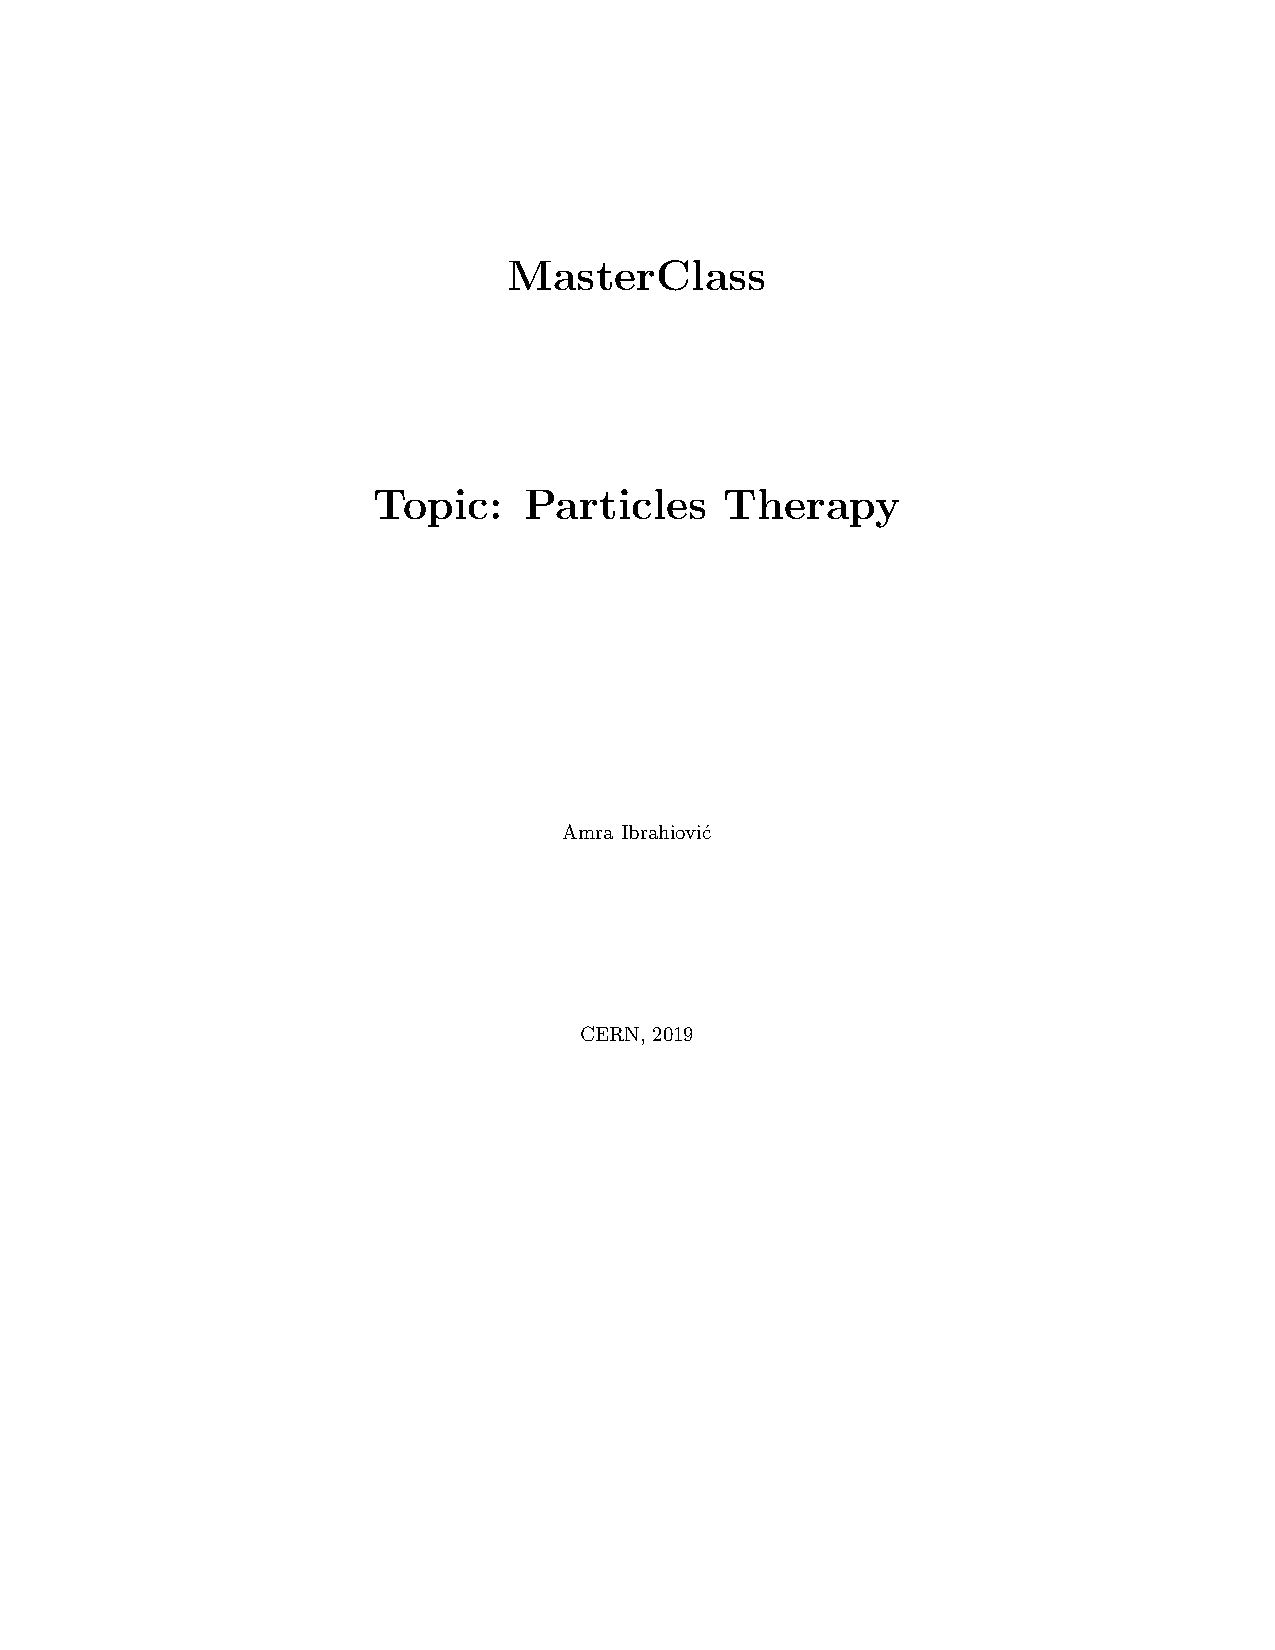
\includegraphics[width = 6cm]{images/Radiotherapy.jpg}
        \caption{caption.}
        \label{fig:1}
    \end{figure}

    \subsection{ფბე (ფარდობითი ბიოლოგიური ეფექტურობა) RBE (relative biological effectiveness)} 
როგორც უკვე ავღნიშნეთ სხვადასხვა ტიპის გამოსხივება სხვადასხვა რაოდენობის გამოსხივებას ტოვებს ბიოლოგიურ ქსოვილებში. ფბე (ფარდობითი ბიოლოგიური ეფექტურება) არის ფარდობითი ზომა რადიიცის დაზიანების
რეფერენს რადიაცია ჩვეულებრივ არის 220 


	\begin{figure}[htp]
	    \centering
        \includegraphics[width = 8cm]{images/Picture1.png}
        \caption{caption.}
        \label{fig:1}
    \end{figure}

\section{რადიაციული თერაპიის დაგეგმვა (Radiation Treatment Planing)}
\subsection{ფანტომები (Phantoms)}
ძირითადი დოზების განაწილების მონაცემები გაზომილია წყლის ფანტომში (water phantom), რომელიც საკმაოდ ახლოსაა კუნთისა და სხვა რბილი რადიაციული შთანთქმის და გაფანტვის რეალურ მნიშვნელობებთან. კიდევ მიზეზი რის გამოც ირჩევენ წყლის ფანტომს, იგი უნივერსალურია და ადვილად შეიძლება რადიციული თვისებების გამეორება (?) [Another reason for the choice of water as a phantom material is that it is universally available with reproducible radiation properties]. რამდენადაც ყოველთვის არაა შესაძლებელი გამოსხივების დეტექტორების წყალში განთავსება, არსებობს მყარი ფანტომები რომლებსაც შეუძლიათ ჩაანაცვლონ წყალი. იდეალურ შემთხვევაში მოცემულ ნივთიერებას რომ იყოს ქსოვილების ანდა წყლის ექვივალენტი, მას უნდა გააჩნდეს იგივე: ეფექტური ატომური რიცხვი, ელექტრონების რიცხვი თითოეულ გრამ ნივთიერებაზე და მასური სიმკვრივე. თუმცა, რადგან კომპტონის ეფექტი არის ძირითადი ურთიერთქმედება მეგავოლტიანი ფოტონების (photon beams in the clinical range,) ნაკადისთვის. ასე შემთხვევაში რომ იყოს ნივთიერება წყლის ექვივალენტი საჭიროა ქონდეს იგივე ელექტრონული სიმკვრივე (ელექტრონების რაოდენობა კუბურ სანტიმეტრზე).
%		\begin{figure}[h]
%		   \centering
%           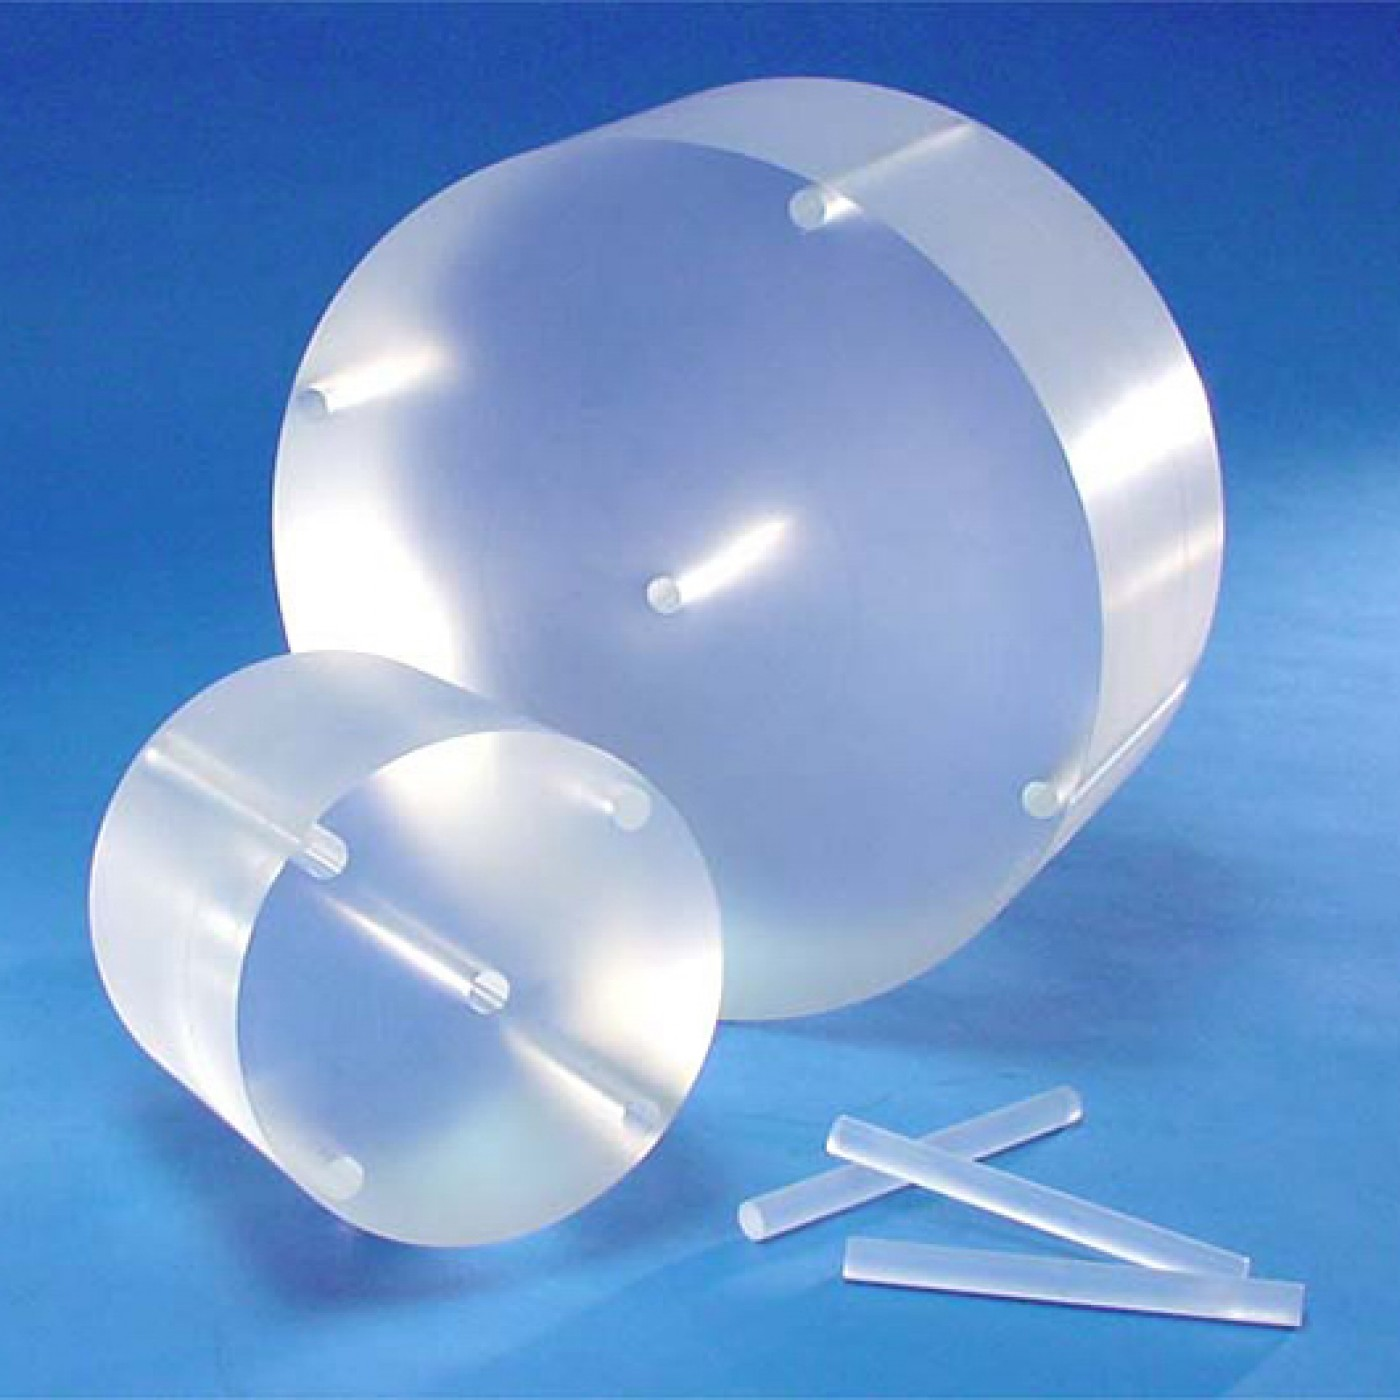
\includegraphics[width=0.4\columnwidth]{images/phantom_a}
%           \caption{სხივთა სვლა თხელ ა) შემკრებ, ბ) გამბნევ ლინზაში.}
%           \label{fig:phantom_a}
%        \end{figure}

	\begin{figure}[h]%
    	\centering
    	\subfloat[\centering მყარი ფანტომი]{{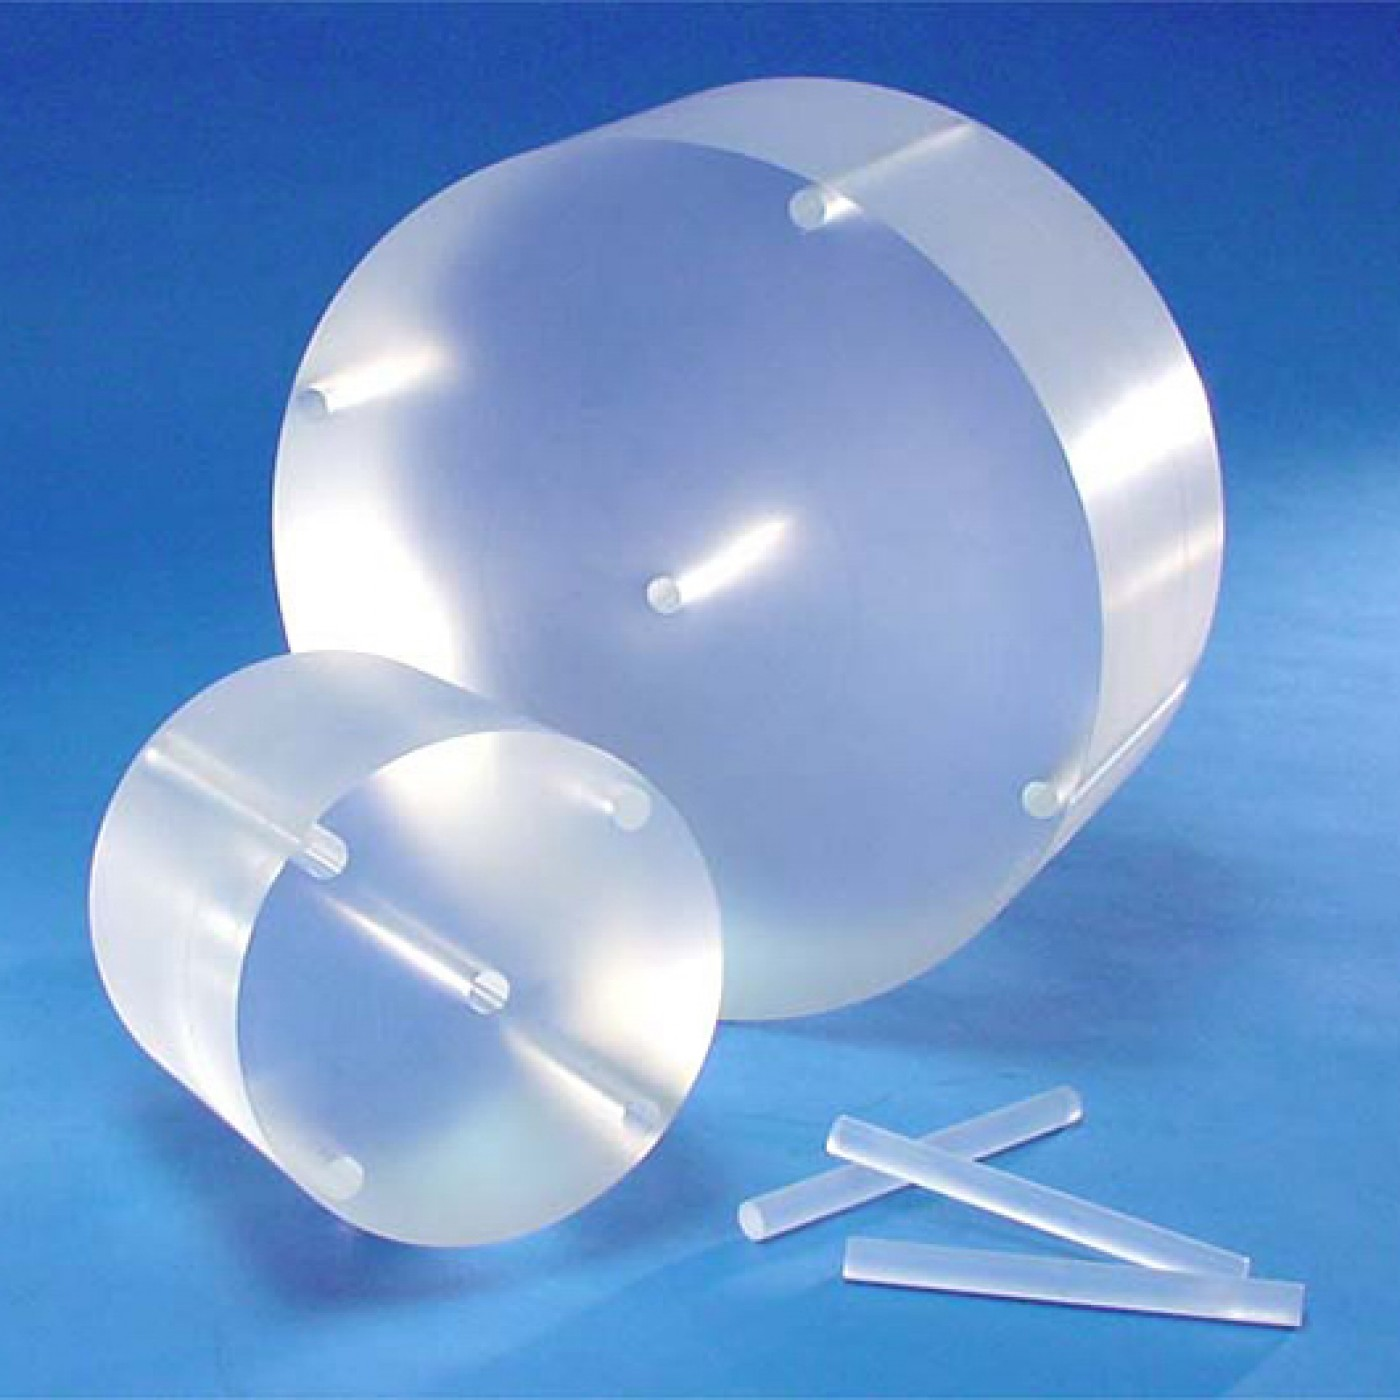
\includegraphics[width=4cm]{images/phantom_a} }}%
    	\qquad
    	\subfloat[\centering წყლის ფანტომი]{{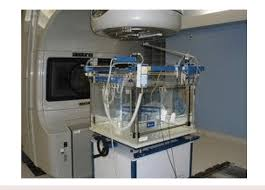
\includegraphics[width=6cm]{images/phantom_b} }}%
    	\caption{ფანტომები}%
    	\label{fig:phantom}%
	\end{figure}
\subsection{მინიმალური სამიზნე დოზა (Minimum Target Dose)}
მინიმალური სამიზნე დოზა არის სამიზნე ფართობის მიერ მინიმალური შთანთქმული დოზა.

\subsection{საშუალო სამიზნე დოზა (Media Target Dose)}
საშუალო სამიზნე დოზა არის სამიზნის მიერ შთანთქმული მაქსიმალური და მინიმალური დოზის საშუალო მნიშვნელობისა.  

\subsection{ცხელი წერტილები (Hot Spots)}
ცხელი წერტილი არის ფართობი რომელიც არის მიზნის გარეთ და იღებს უფრო მეტ დოზას ვიდრე მიზნისთვისაა განსაზღვრული. როგორც მაქსიმალური სამიზნე დოზა, ცხელი წერტილი იძენს სამედიცინო აზრს თუ ის ფარავს სულ მცირე 2~$\text{სმ}^2$ ფართობს.

\subsection{მონაცემთა მოგროვება (Data Acquisition)}


\section{თანამედროვე რადიაციული თერაპია (Modern Radiation Therapy)}



\chapter{მითითებები}

\chapter{პროტონული ნაკადებით თერაპია}
პროტონების საშუალებით რადიოთერაპიული მკურნალობის დაგეგვმის ძირითადი პრინციპი იგივეა რაც ფოტონებისათვის და ელექტრონებისთვის. უნდა მოვაგროვოთ მოცულობითი გამოსახულება
\medskip

\bibliography{bibliography.bib} 

\end{document}